\documentclass[tikz,border=10pt]{standalone}
\usepackage{amsmath}
\begin{document}
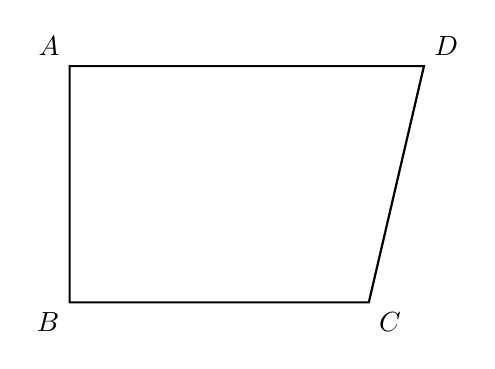
\begin{tikzpicture}[thick, scale=1]
  \coordinate (A) at (0,3);
  \coordinate (D) at (4.5,3);
  \coordinate (C) at (3.8,0);
  \coordinate (B) at (0,0);

  \draw (A) -- (D) -- (C) -- (B) -- cycle;

  \node[above left] at (A) {$A$};
  \node[above right] at (D) {$D$};
  \node[below right] at (C) {$C$};
  \node[below left] at (B) {$B$};
\end{tikzpicture}
\end{document}
